%%%
% Plantilla de Memoria
% Modificación de una plantilla de Latex de Nicolas Diaz para adaptarla 
% al castellano y a las necesidades de escribir informática y matemáticas.
%
% Editada por: Mario Román
%
% License:
% CC BY-NC-SA 3.0 (http://creativecommons.org/licenses/by-nc-sa/3.0/)
%%%

%%%%%%%%%%%%%%%%%%%%%%%%%%%%%%%%%%%%%%%%%
% Thin Sectioned Essay
% LaTeX Template
% Version 1.0 (3/8/13)
%
% This template has been downloaded from:
% http://www.LaTeXTemplates.com
%
% Original Author:
% Nicolas Diaz (nsdiaz@uc.cl) with extensive modifications by:
% Vel (vel@latextemplates.com)
%
% License:
% CC BY-NC-SA 3.0 (http://creativecommons.org/licenses/by-nc-sa/3.0/)
%
%%%%%%%%%%%%%%%%%%%%%%%%%%%%%%%%%%%%%%%%%

%----------------------------------------------------------------------------------------
%	PAQUETES Y CONFIGURACIÓN DEL DOCUMENTO
%----------------------------------------------------------------------------------------
%%% Configuración del papel.
% microtype: Tipografía.
% mathpazo: Usa la fuente Palatino.
\documentclass[a4paper, 11pt]{article}
\usepackage[protrusion=true,expansion=true]{microtype}
\usepackage{mathpazo}

\usepackage{fancyvrb}

% redefine \VerbatimInput
\RecustomVerbatimCommand{\VerbatimInput}{VerbatimInput}%
{fontsize=\footnotesize,
	%
	frame=lines,  % top and bottom rule only
	framesep=2em, % separation between frame and text
	rulecolor=\color{Gray},
	%
	label=\fbox{\color{Black}data.txt},
	labelposition=topline,
	%
	commandchars=\|\(\), % escape character and argument delimiters for
	% commands within the verbatim
	commentchar=*        % comment character
}


\usepackage{movie15}


% Indentación de párrafos para Palatino
\setlength{\parindent}{0pt}
  \parskip=8pt
\linespread{1.05} % Change line spacing here, Palatino benefits from a slight increase by default




%%% Castellano.
% noquoting: Permite uso de comillas no españolas.
% lcroman: Permite la enumeración con numerales romanos en minúscula.
% fontenc: Usa la fuente completa para que pueda copiarse correctamente del pdf.
\usepackage[spanish,es-noquoting,es-lcroman]{babel}
\usepackage[utf8]{inputenc}
\usepackage[T1]{fontenc}
\selectlanguage{spanish}




%%% Gráficos
\usepackage{graphicx} % Required for including pictures
\usepackage{wrapfig} % Allows in-line images
\usepackage[usenames,dvipsnames]{color} % Coloring code
\usepackage{graphicx}

%%% Matemáticas
\usepackage{amsmath}


%%% Bibliografía
\makeatletter
\renewcommand\@biblabel[1]{\textbf{#1.}} % Change the square brackets for each bibliography item from '[1]' to '1.'
\renewcommand{\@listI}{\itemsep=0pt} % Reduce the space between items in the itemize and enumerate environments and the bibliography


%% codigo

%%% CÓDIGO
 \usepackage{listings}
\usepackage{courier}
\lstset{
	basicstyle=\footnotesize\ttfamily, % Standardschrift
	numbers=left,               % Ort der Zeilennummern
	numberstyle=\tiny,          % Stil der Zeilennummern
	stepnumber=1,               % Abstand zwischen den Zeilennummern
	numbersep=5pt,              % Abstand der Nummern zum Text
	tabsize=2,                  % Groesse von Tabs
	extendedchars=true,         %
	breaklines=true,            % Zeilen werden Umgebrochen
	keywordstyle=\color{red},
	frame=b,         
	%        keywordstyle=[1]\textbf,    % Stil der Keywords
	%        keywordstyle=[2]\textbf,    %
	%        keywordstyle=[3]\textbf,    %
	%        keywordstyle=[4]\textbf,   \sqrt{\sqrt{}} %
	stringstyle=\color{white}\ttfamily, % Farbe der String
	showspaces=false,           % Leerzeichen anzeigen ?
	showtabs=false,             % Tabs anzeigen ?
	xleftmargin=17pt,
	framexleftmargin=17pt,
	framexrightmargin=5pt,
	framexbottommargin=4pt,
	%backgroundcolor=\color{lightgray}
	showstringspaces=false      % Leerzeichen in Strings anzeigen ?        
	literate=
	{á}{{\'a}}1 {é}{{\'e}}1 {í}{{\'i}}1 {ó}{{\'o}}1 {ú}{{\'u}}1
	{Á}{{\'A}}1 {É}{{\'E}}1 {Í}{{\'I}}1 {Ó}{{\'O}}1 {Ú}{{\'U}}1
	{à}{{\`a}}1 {è}{{\`e}}1 {ì}{{\`i}}1 {ò}{{\`o}}1 {ù}{{\`u}}1
	{À}{{\`A}}1 {È}{{\'E}}1 {Ì}{{\`I}}1 {Ò}{{\`O}}1 {Ù}{{\`U}}1
	{ä}{{\"a}}1 {ë}{{\"e}}1 {ï}{{\"i}}1 {ö}{{\"o}}1 {ü}{{\"u}}1
	{Ä}{{\"A}}1 {Ë}{{\"E}}1 {Ï}{{\"I}}1 {Ö}{{\"O}}1 {Ü}{{\"U}}1
	{â}{{\^a}}1 {ê}{{\^e}}1 {î}{{\^i}}1 {ô}{{\^o}}1 {û}{{\^u}}1
	{Â}{{\^A}}1 {Ê}{{\^E}}1 {Î}{{\^I}}1 {Ô}{{\^O}}1 {Û}{{\^U}}1
	{œ}{{\oe}}1 {Œ}{{\OE}}1 {æ}{{\ae}}1 {Æ}{{\AE}}1 {ß}{{\ss}}1
	{ű}{{\H{u}}}1 {Ű}{{\H{U}}}1 {ő}{{\H{o}}}1 {Ő}{{\H{O}}}1
	{ç}{{\c c}}1 {Ç}{{\c C}}1 {ø}{{\o}}1 {å}{{\r a}}1 {Å}{{\r A}}1
	{€}{{\euro}}1 {£}{{\pounds}}1 {«}{{\guillemotleft}}1
	{»}{{\guillemotright}}1 {ñ}{{\~n}}1 {Ñ}{{\~N}}1 {¿}{{?`}}1   
}


\lstloadlanguages{% Check Dokumentation for further languages ...
%[Visual]Basic
%Pascal
%C
C++
%%XML
%%HTML
%Java
}
%\DeclareCaptionFont{blue}{\color{blue}} 

%\captionsetup[lstlisting]{singlelinecheck=false, labelfont={blue}, textfont={blue}}
\usepackage{caption}
\DeclareCaptionFont{white}{\color{white}}
\DeclareCaptionFormat{listing}{\colorbox[cmyk]{0.43, 0.35, 0.35,0.01}{\parbox{\textwidth}{\hspace{15pt}#1#2#3}}}
\captionsetup[lstlisting]{format=listing,labelfont=white,textfont=white, singlelinecheck=false, margin=0pt, font={bf,footnotesize}
}

%% cosas 

\usepackage[margin=1in]{geometry}

\usepackage{times}


%% colorear titulos
\usepackage{titlesec}
\titleformat{\section}
{\color{azulillo}\normalfont\Large\bfseries}
{\color{Black}\thesection}{1em}{}


%% ENLACES 
\usepackage{hyperref}
\hypersetup{
	colorlinks   = true,    % Colours links instead of ugly boxes
	urlcolor     = black,    % Colour for external hyperlinks
	linkcolor    = black, %BurntOrange,    % Colour of internal links
	citecolor    = black      % Colour of citations
}


%% CREAR DIAGRAMAS 

\usepackage{tikz}

%% rodear figura de texto
\usepackage{graphicx,wrapfig,lipsum}
 %% comentarios multilinea
\usepackage{verbatim}

\definecolor{darkGray}{gray}{0.05}
\usepackage{animate}
\definecolor{rojizo}{RGB}{217, 83, 79}
\definecolor{azulillo}{RGB}{79, 83, 217}

%----------------------------------------------------------------------------------------
%	DOCUMENTO
%----------------------------------------------------------------------------------------

\begin{document}
	
	
	\begin{titlepage}
		\begin{center}
			\vspace*{0.2cm}
			
			{\Huge \textbf{\textcolor{azulillo}{Recubrimiento de un grafo por vértices (Recorrido del caballo.)}}}
			
						{\textcolor{black}	{\Huge\underline{practica 4: BÚSQUEDA}}}
			
				\vspace{0.2cm}
				
				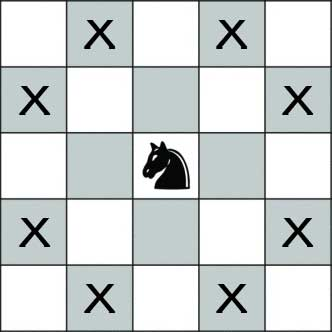
\includegraphics[width=0.8\textwidth]{cover.jpg}
				\vspace{0.2cm}
				

		
			\vspace{1cm}
			
			\textbf{AUTORES: \\
					Pablo Moreno Megías, Diego Lerena García, Manuel Vallejo Felipe, Ángel Díaz de la Torre, Francisco Navarro Morales, Marcel Kemp Muñoz y David Redondo Correa
		    		 }
	    		 \vspace{1cm}
	   
			
			\vfill
			Algorítmica [PRACTICAS]\\
			Segundo curso del Grado de Ingeniería Informática.\\
			Universidad de Granada.\\
			curso 2016-2017.
		\end{center}
	\end{titlepage}


%\maketitle % Print the title section

%% Resumen (Descomentar para usarlo)
\renewcommand{\abstractname}{Resumen} % Uncomment to change the name of the abstract to something else
%\begin{abstract}
% Resumen aquí
%\end{abstract}

%% Palabras clave
%\hspace*{3,6mm}\textit{Keywords:} lorem , ipsum , dolor , sit amet , lectus % Keywords
%\vspace{30pt} % Some vertical space between the abstract and first section

\color{darkGray}
%% Índice
{\parskip=2pt
  \tableofcontents
}
\pagebreak

\section{Análisis del problema}



Se tiene un  tablero de Ajedrez y se sitúa un caballo solitario en cualquier casilla de este y se quiere, utilizando la reglas del juego, que el caballo recorra todas y cada una de las casillas del tablero sin repetir ninguna casilla visitada.

	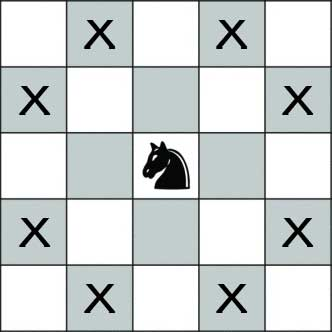
\includegraphics[width=0.5\textwidth]{cover.jpg}
		
				Si observamos la figura y enmueramos, definimos y ordenamos los movimientos del cabllao de ajedrez (1-8), tomando el primer movimiento como el superior más a la de la izquierda y siguiendo un sentido horario tenemos los 8 movimientos del cabllo de ajedrez desde una posición (xk,ym) de un tablero cuadrado hacia una posición (xk+1,ym+1), convirtiendo el propio tablero en un sistema de coordenadas cartesianas o un mapa:
			
				posición 1: se le restan 2 posiciones a la x y se le suma una 1posicion a la y
				
				posición 2: se le resta 1 a la x y se le suman 2 a la y
				
				posición 3: se le suma 1 a la x y se le suman 2 a la y
				
				posición 4: se le suman 2 a la x y se le suma 1 a la y
				
				posición 5: se le suman 2 a la x y se le resta 1 a la y
				
				posición 6: se le suma 1 a la x y se le restan 2 a la y
				
				posición 7: se le resta 1 a la x y se le restan 2 a la y
				
				posición 8: se le restan 2 a la x y se le resta 1 a la y 
				
				No hace falta decir que un movimiento es válido si y solo si el movimiento está dentro del tablero, pues entonces tenemos que tener cuidado en los bordes.
				
				En casos de un tablero de dimensiones menores a 4x4 es posible que se dé el caso de que sea irresoluble el problema debido al propio movimiento del caballo.

\section{Escoger una técnica (BackTracking o Branch and Bound) y justificar su elección frente a la otra metodología no seleccionada.}	
La técnica que hemos elegido para el problema del recorrido del caballo ha sido Backtracking

¿Por qué no Brach and Bound?
Somos conscientes de que se puede resolver mucho más eficiente con Branch and Bound y que quizá utilizar branch and bound sea poco práctico teniendo en cuenta la cantidad de recorridos posibles para el caballo en un tablero 8x8. No obstante, es muy complicado establecer la bondad de un nodo o una estrategia de ramificación tan buena para que vaya podando y puede ser que vaya dejando soluciones que pueden ser factibles (si no lo hacemos con una estimación óptima).
Un solución para ello sería algo parecido a un pathfinding realizado en las prácticas de IA. Si fusionamos esos dos conceptos obtendríamos un resultado preferible, pero encontrar un criterio que permita implementar una solución Branch and Bound es algo complejo que, probablemente, escape a los objetivos de esta asignatura.

Por ello, nos decantamos por Backtracking que aunque es menos eficiente y por consiguiente tarda más tiempo en determinar si hay solución o no, lo resuelve en tiempo razonable (que es el objetivo) y además es bastante más rápido de implementar y con tres parciales y dos finales a la vuelta de la esquina no era plan de ponerse a hacer el mongolo pensando una solución Branch and Bound.

\section{Diseño de la solución, describiendo cada una de las componentes de la misma relacionándola con las componentes de un algoritmo BackTracking o Branch\&Bound, según la técnica escogida.}
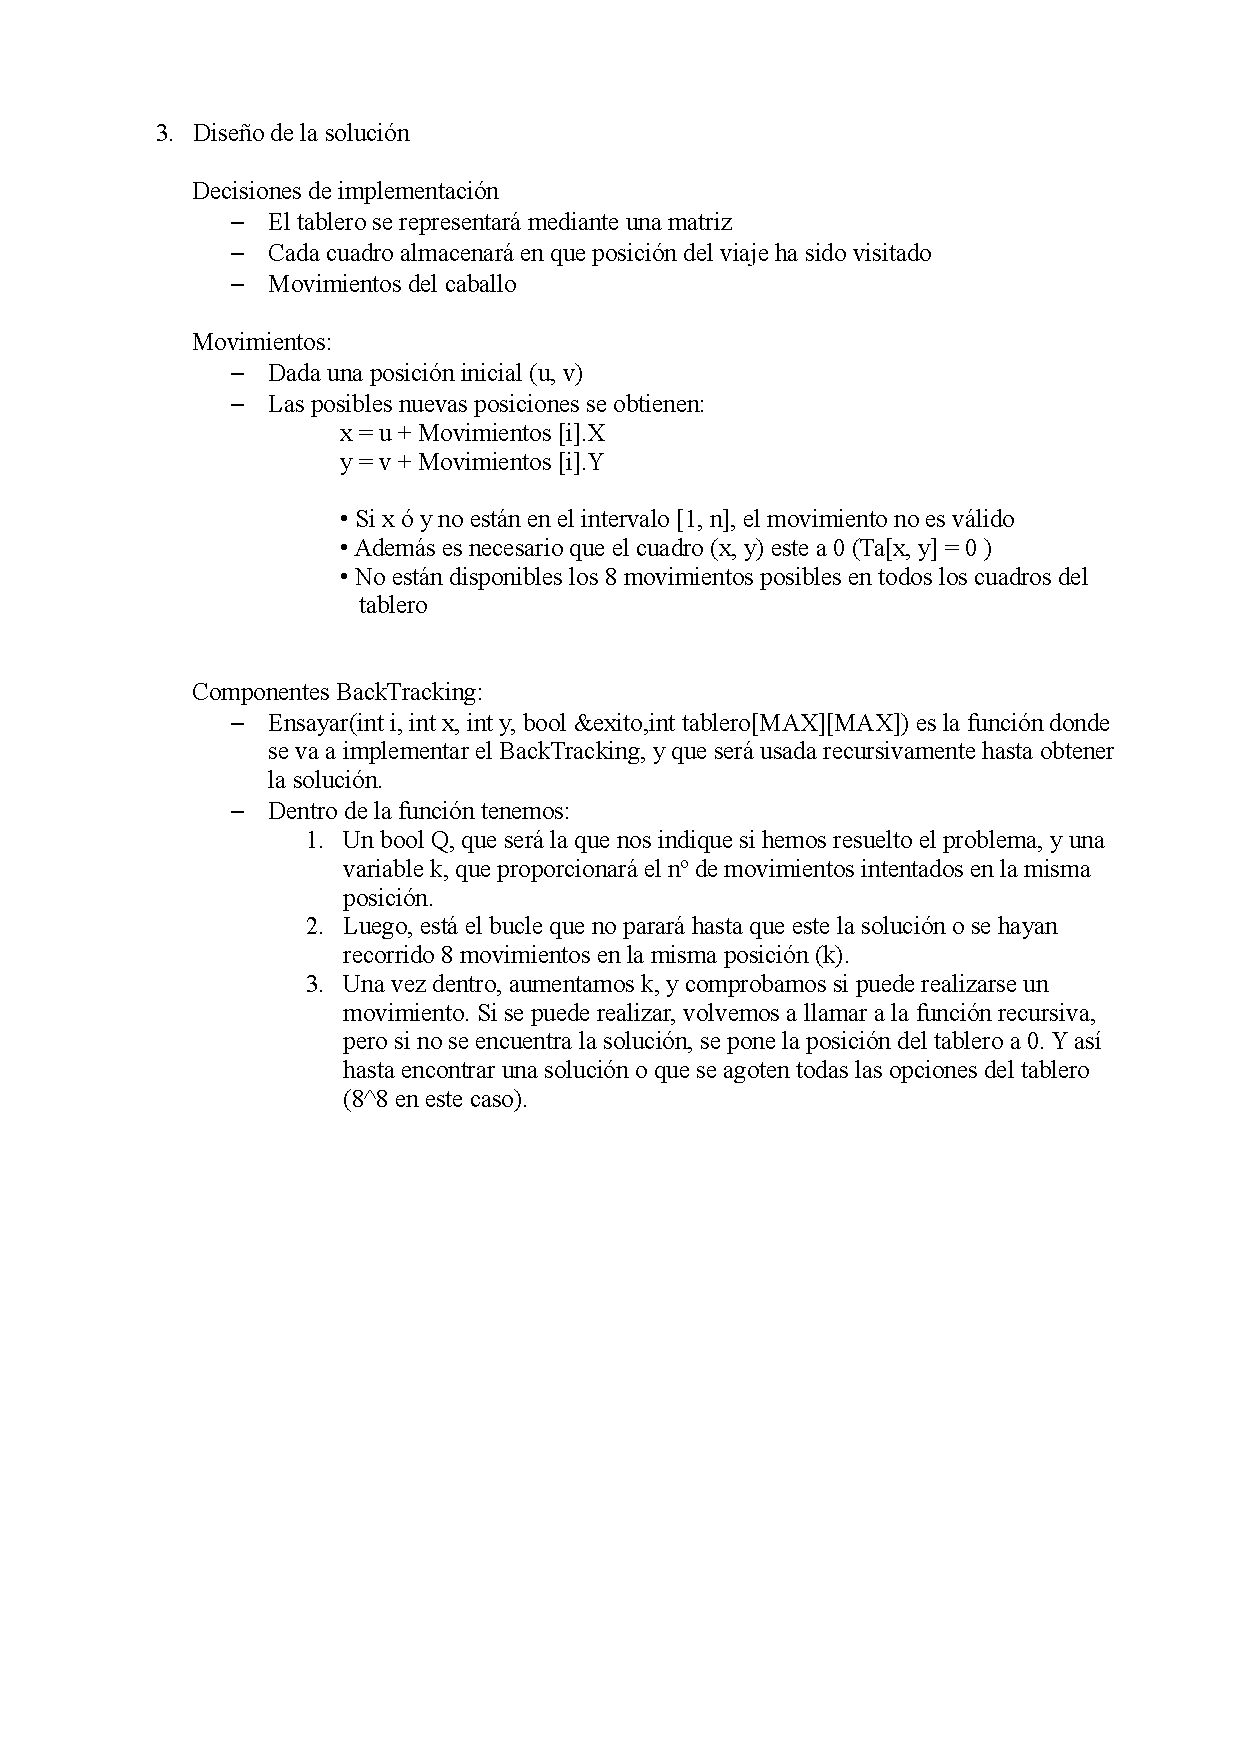
\includegraphics[width=\textwidth]{sol.pdf}

\section{Esqueleto del algoritmo (pseudocódigo) que soluciona el problema, explicando cómo se ha incorporado cada una de las componentes de diseño de la técnica (BackTracking o Branch\&Bound, según se aplique)}

	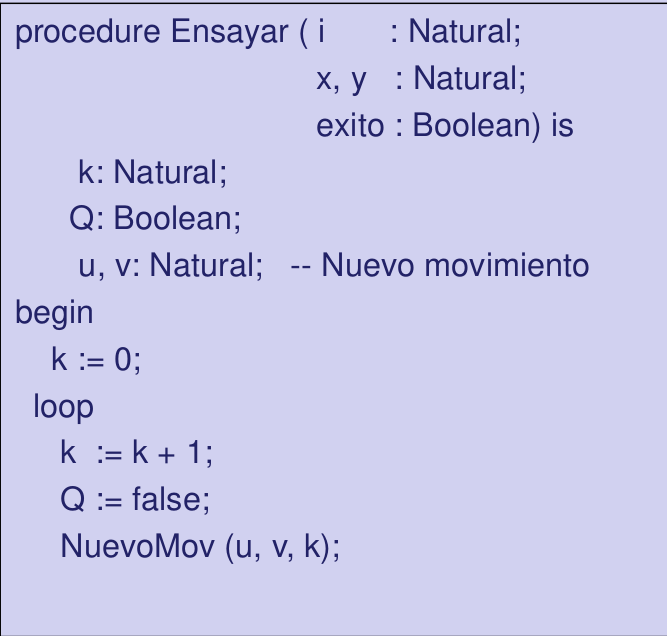
\includegraphics[width=0.4\textwidth]{asd.png}
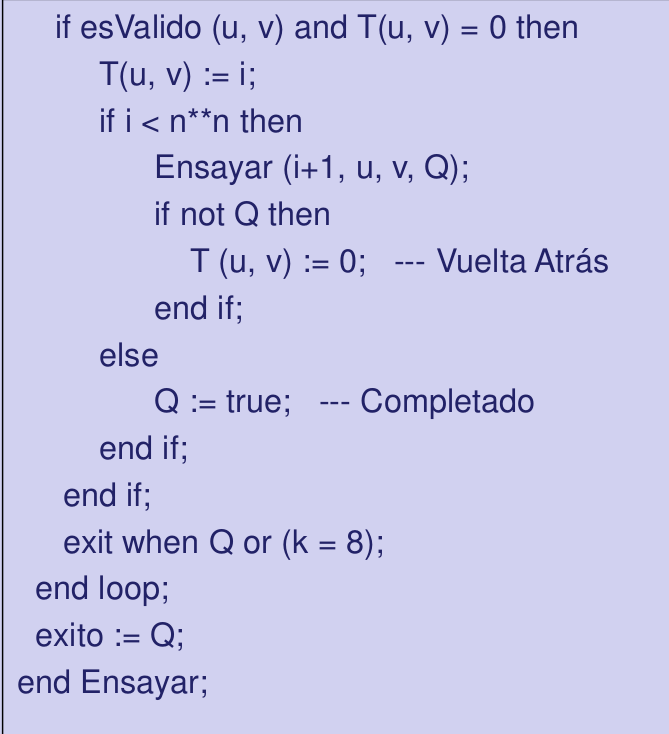
\includegraphics[width=0.4\textwidth]{asd2.png}
								
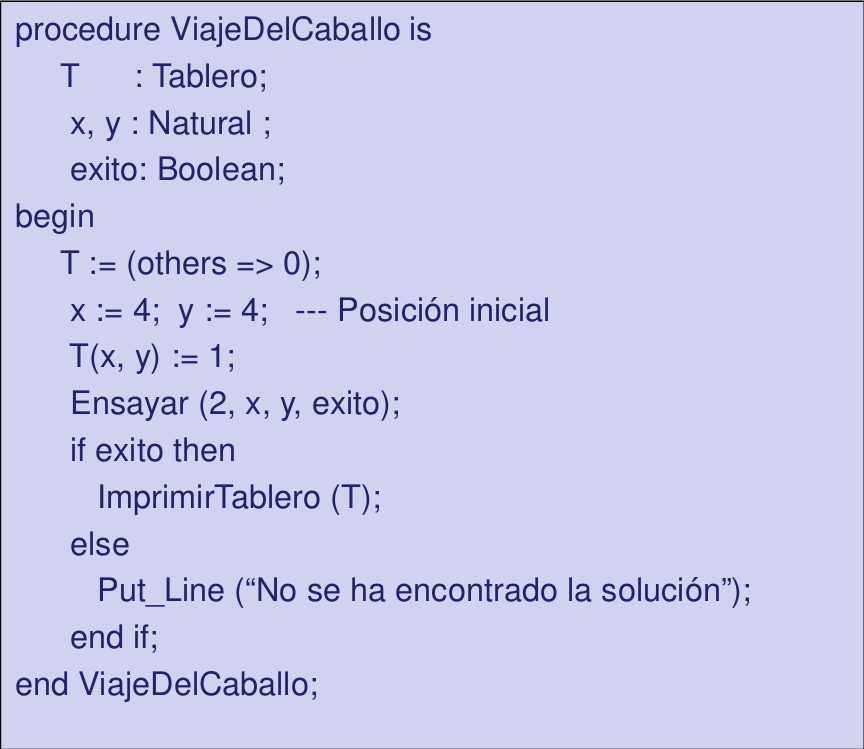
\includegraphics[width=0.8\textwidth]{asd3.png}


\section{Explicación del funcionamiento del algoritmo, sobre un caso de ejemplo pequeño propuesto por los estudiantes.}

El algoritmo comienza con el caballo colocado en la casilla que se le indique, a la que se le asigna el número 1. A continuación va calculando las casillas resultantes de efectuar cada uno de los 8 posibles movimientos, si el movimiento que calcula para un movimiento es válido (lleva a una casilla del tablero que aún no ha sido visitada) vuelve a llamar a la función y avanza. En caso de no encontrar ningún movimiento válido para una posición concreta, el algoritmo retrocede, marca un 0 en la última posición válida que se había calculado y sigue calculando sus hermanos. Para ello utiliza una matriz rellena a -1 (representa que la casilla no ha sido visitada) qie va rellenando con el turno o momento en el que el caballo se encuentra en cada casilla. Ejemplo de ejecución para un tablero 3x3: 

				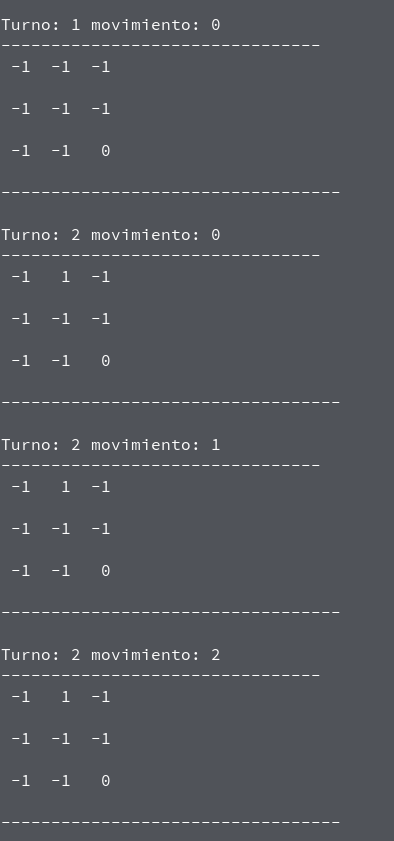
\includegraphics[width=0.33\textwidth]{a.png}
				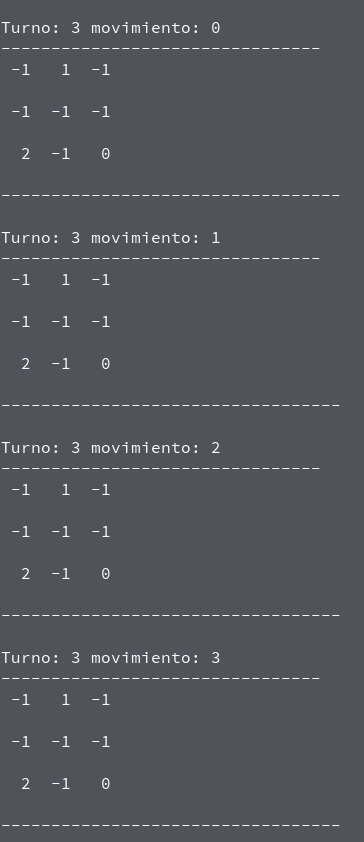
\includegraphics[width=0.33\textwidth]{b.png}								
				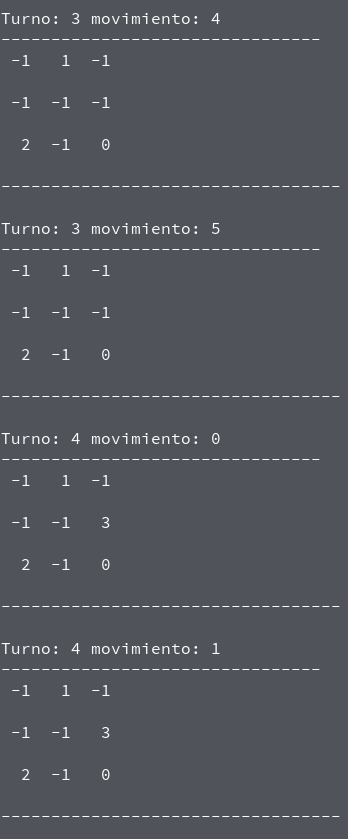
\includegraphics[width=0.33\textwidth]{c.png}
				
				...
				
				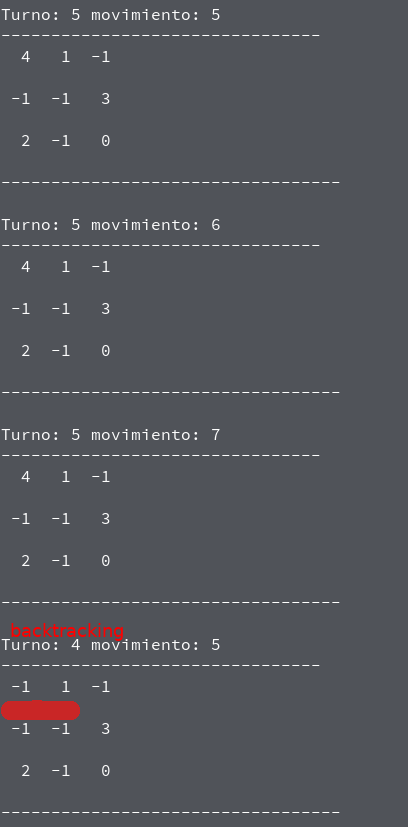
\includegraphics[width=0.33\textwidth]{d.png}
				



\section{Enunciado de un problema o caso real donde se pueda utilizar la técnica seleccionada para solucionarlo (distinto de los comentados en clase).}
El algoritmo sirve para resolver el famoso problema del movimiento del caballo en el juego del ajedrez. El esquema que utiliza se puede extrapolar para resolver otros problemas de búsqueda pero estaríamos hablando del esquema branch and bound típico, puesto que este no tiene nada de especial.

\section{Cálculo del orden de eficiencia teórico del algoritmo.}

El algoritmo prueba todos los caminos posibles hasta que encuentra uno válido. Suponiendo que tuviera que probar todos los caminos posibles:
Como en total el caballo tiene que visitar $MAX\times MAX$ casillas (sea $MAX,\ n$, $n^2$ casillas)...

Si suponemos que de cada nodo surgen siempre 5 nodos válidos (para establecer una aproximación, podría darse que un nodo tuviera 8 hijos válidos o incluso 0 hijos válidos) y dado que el nivel del árbol de búsqueda debe ser $n^2$ (un nivel por cada posición posible del tablero), como de cada nodo suponemos que salen 5 nodos, de la raíz se obtienen 5 nodos, de cada uno de esos nodos se obtienen otros 5 (en total 25) y de cada uno de esos 25, otros 5... es decir, que en total se evaluarían $5^x$ nodos siendo x el nivel del nodo, como $x=n^2$, el número de nodos a evaluar sería $5^{n^2}=5^{2n}$ que, para un tablero 8x8 sería un total de $5^16=152587890625$ nodos, si el número de nodos válidos fuera mayor, por ejemplo 8 (que sería una buena cota superior porque es imposible que todos los nodos den siempre 8 hijos válidos) se obtendría un total de $2.814749767\times 10{14}$ nodos.

En conclusión, suponiendo que cada nodo se evalúa en $O(1)$, la eficiencia teórica del algoritmo sería $O(k^{2n})$ donde k es el número medio de hijos válidos por nodo (al principio y dependiendo del tamaño del tablero podrá tomar valores próximos a 8 y en niveles profundos del árbol tomará valores cercanos a 0, por lo que una buena aproximación sería 4 o 5).




\section{8. Instrucciones sobre cómo compilar y ejecutar el código de la práctica.}

El código es un .cpp, se compila con g++ sin ningún parámetro especial necesario. 
Si se desea modificar la casilla inicial o el tamaño del tablero basta con modificar los valores de las variables x e y en el main o de la constante global MAX (que representa el número de filas y de columnas del tablero).

El código por defecto se ejecuta en un tablero 7x7 porque la solución es inmediata. En un tablero 8x8 tarda unas horas en encontrar la respuesta, pero la encuentra.

Algunas ejecuciones con distintos tamaños:

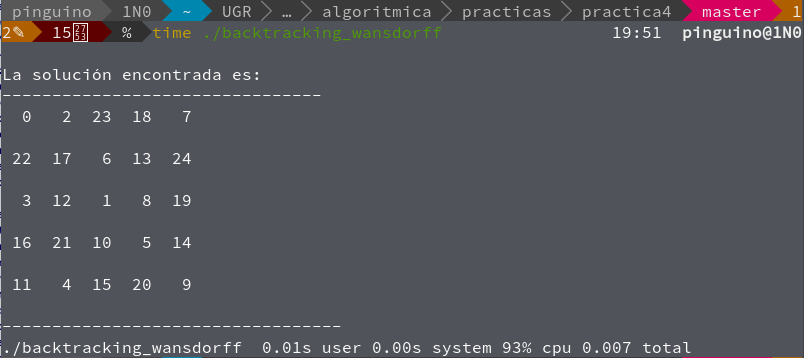
\includegraphics[width=0.8\textwidth]{0.png}

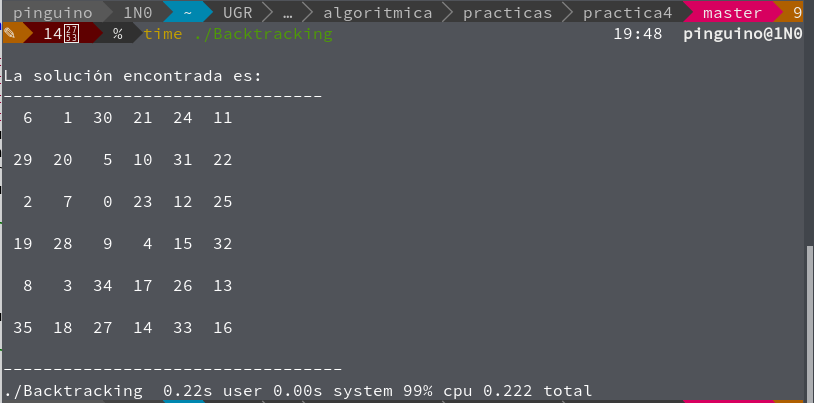
\includegraphics[width=0.8\textwidth]{1.png}								

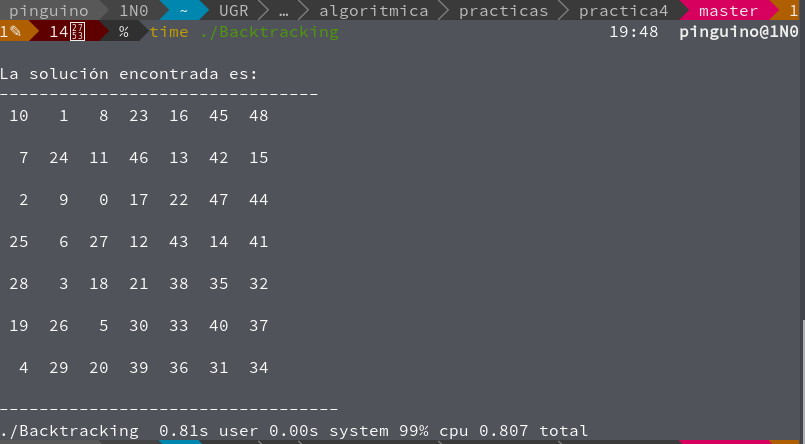
\includegraphics[width=0.8\textwidth]{2.png}

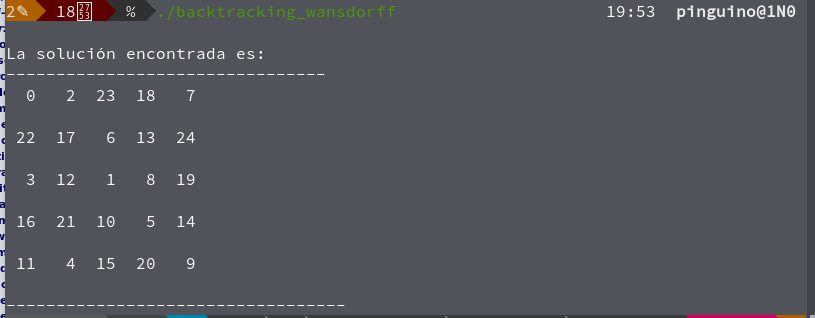
\includegraphics[width=0.8\textwidth]{00.png}

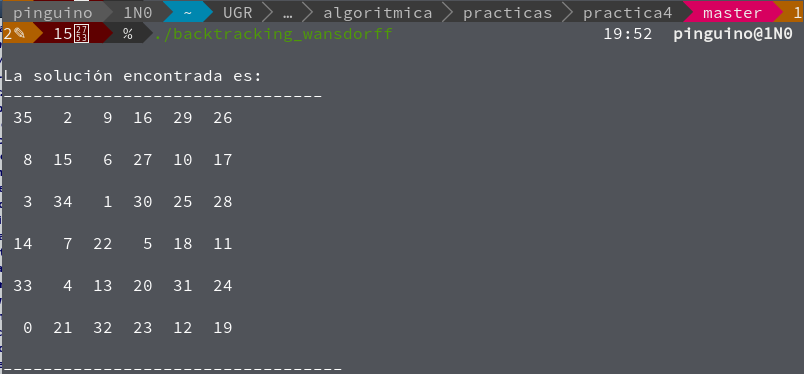
\includegraphics[width=0.8\textwidth]{01.png}								

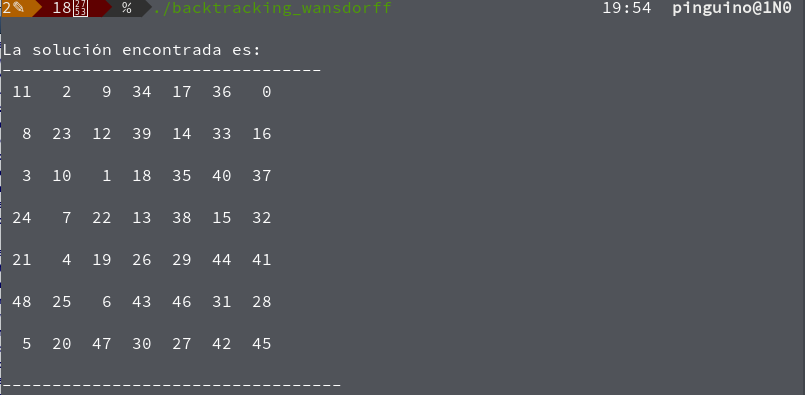
\includegraphics[width=0.8\textwidth]{02.png}

	

\end{document}